\documentclass{article}
\usepackage[polish]{babel}
\usepackage[a4paper, margin=2cm]{geometry}
\usepackage{graphicx}
\usepackage{polski}
\usepackage[utf8]{inputenc}
\usepackage{lettrine}
\usepackage{xcolor}
\usepackage[nodayofweek]{datetime}
\renewcommand{\familydefault}{\sfdefault}

\usepackage[autocite=superscript]{biblatex}
\addbibresource{bibliography.bib}

\title{Wspinaczka sportowa w Polsce: stosowane skale wyceny trudności tras oraz popularne rejony skałkowe}
\author{Marcin Młynarczyk}
\newdate{date}{19}{6}{2020}
\date{\displaydate{date}}
\definecolor{blue}{cmyk}{.6,.28,0,.04}

\usepackage{sectsty}
\chapterfont{\color{blue}}
\sectionfont{\color{blue}}
\subsectionfont{\color{blue}}
\subsubsectionfont{\color{blue}}

\addto\captionspolish{
  \renewcommand{\contentsname}%
    {\color{blue}Spis treści}%
}

\begin{document}

\maketitle
\tableofcontents

\bigskip

\begin{figure}[!htbp]
	\begin{center}
		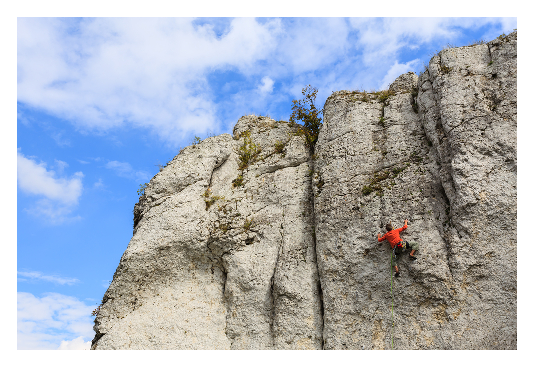
\includegraphics[width=0.9\linewidth]{images/wspin-jura.eps}
	\end{center}
	\caption{Wspinanie w skałach Jury Krakowsko-Częstochowskiej \cite{jura-intro}}
	\label{}
\end{figure}

\section{Wstęp}
%\lettrine[lines=2]{}{}

\section{Stosowane skale wyceny trudności tras sportowych w Polsce}
\lettrine[lines=2]{O}{} piszę w tej pracy dwie najpopularniejsze skale wyceny wspinaczkowych tras sportowych w Polsce - skalę Kurtyki, najczęściej spotykaną w skałach i na niektórych ścianach sztucznych, oraz skalę francuską, która ze względu na większą rozpoznawalność na świecie, spotykana jest na obiektach krytych.

\subsection{Skala Kurtyki}

\subsection{Skala francuska}

\subsection{Skala saksońska}

\subsection{Próba porównania skal}


\section{Popularne rejony skałkowe w Polsce}
\lettrine[lines=2]{W}{} tej części pracy przedstawię kilka rejonów skałkowych w Polsce - począwszy od najpopularniejszej Jury, po mniej znane - Sokoliki i Góry Stołowe.

\subsection{Jura Krakowsko-Częstochowska}
Bez wątpienia jest to najczęściej odwiedzany rejon skałkowy w Polsce. Jednym z powodów owej popularności może być liczność dostępnych skał - jest to bowiem największe skupisko skał wapiennych w naszym kraju. Jura jest wyżyną rozciągającą się pomiędzy Krakowem, a Częstochową. Ze względu na swoją wielkość rejon ten jest z reguły dzielony na część północną, środkową i południową. Na Jurze trasy wyceniane według skali Kurtyki, o której wcześniej już tutaj pisano. Według statystyk na stronie Portalu Górskiego \cite{topo-jura}, na Jurze wytyczono prawie 8900 tras. Największy wybór tras znajdziemy tutaj o wycenie VI.1+ - aż 772 trasy \cite{topo-jura}, ale również bardziej początkujący lub zaawansowani znajdą tutaj coś dla siebie.

\begin{figure}[!htbp]
	\begin{center}
		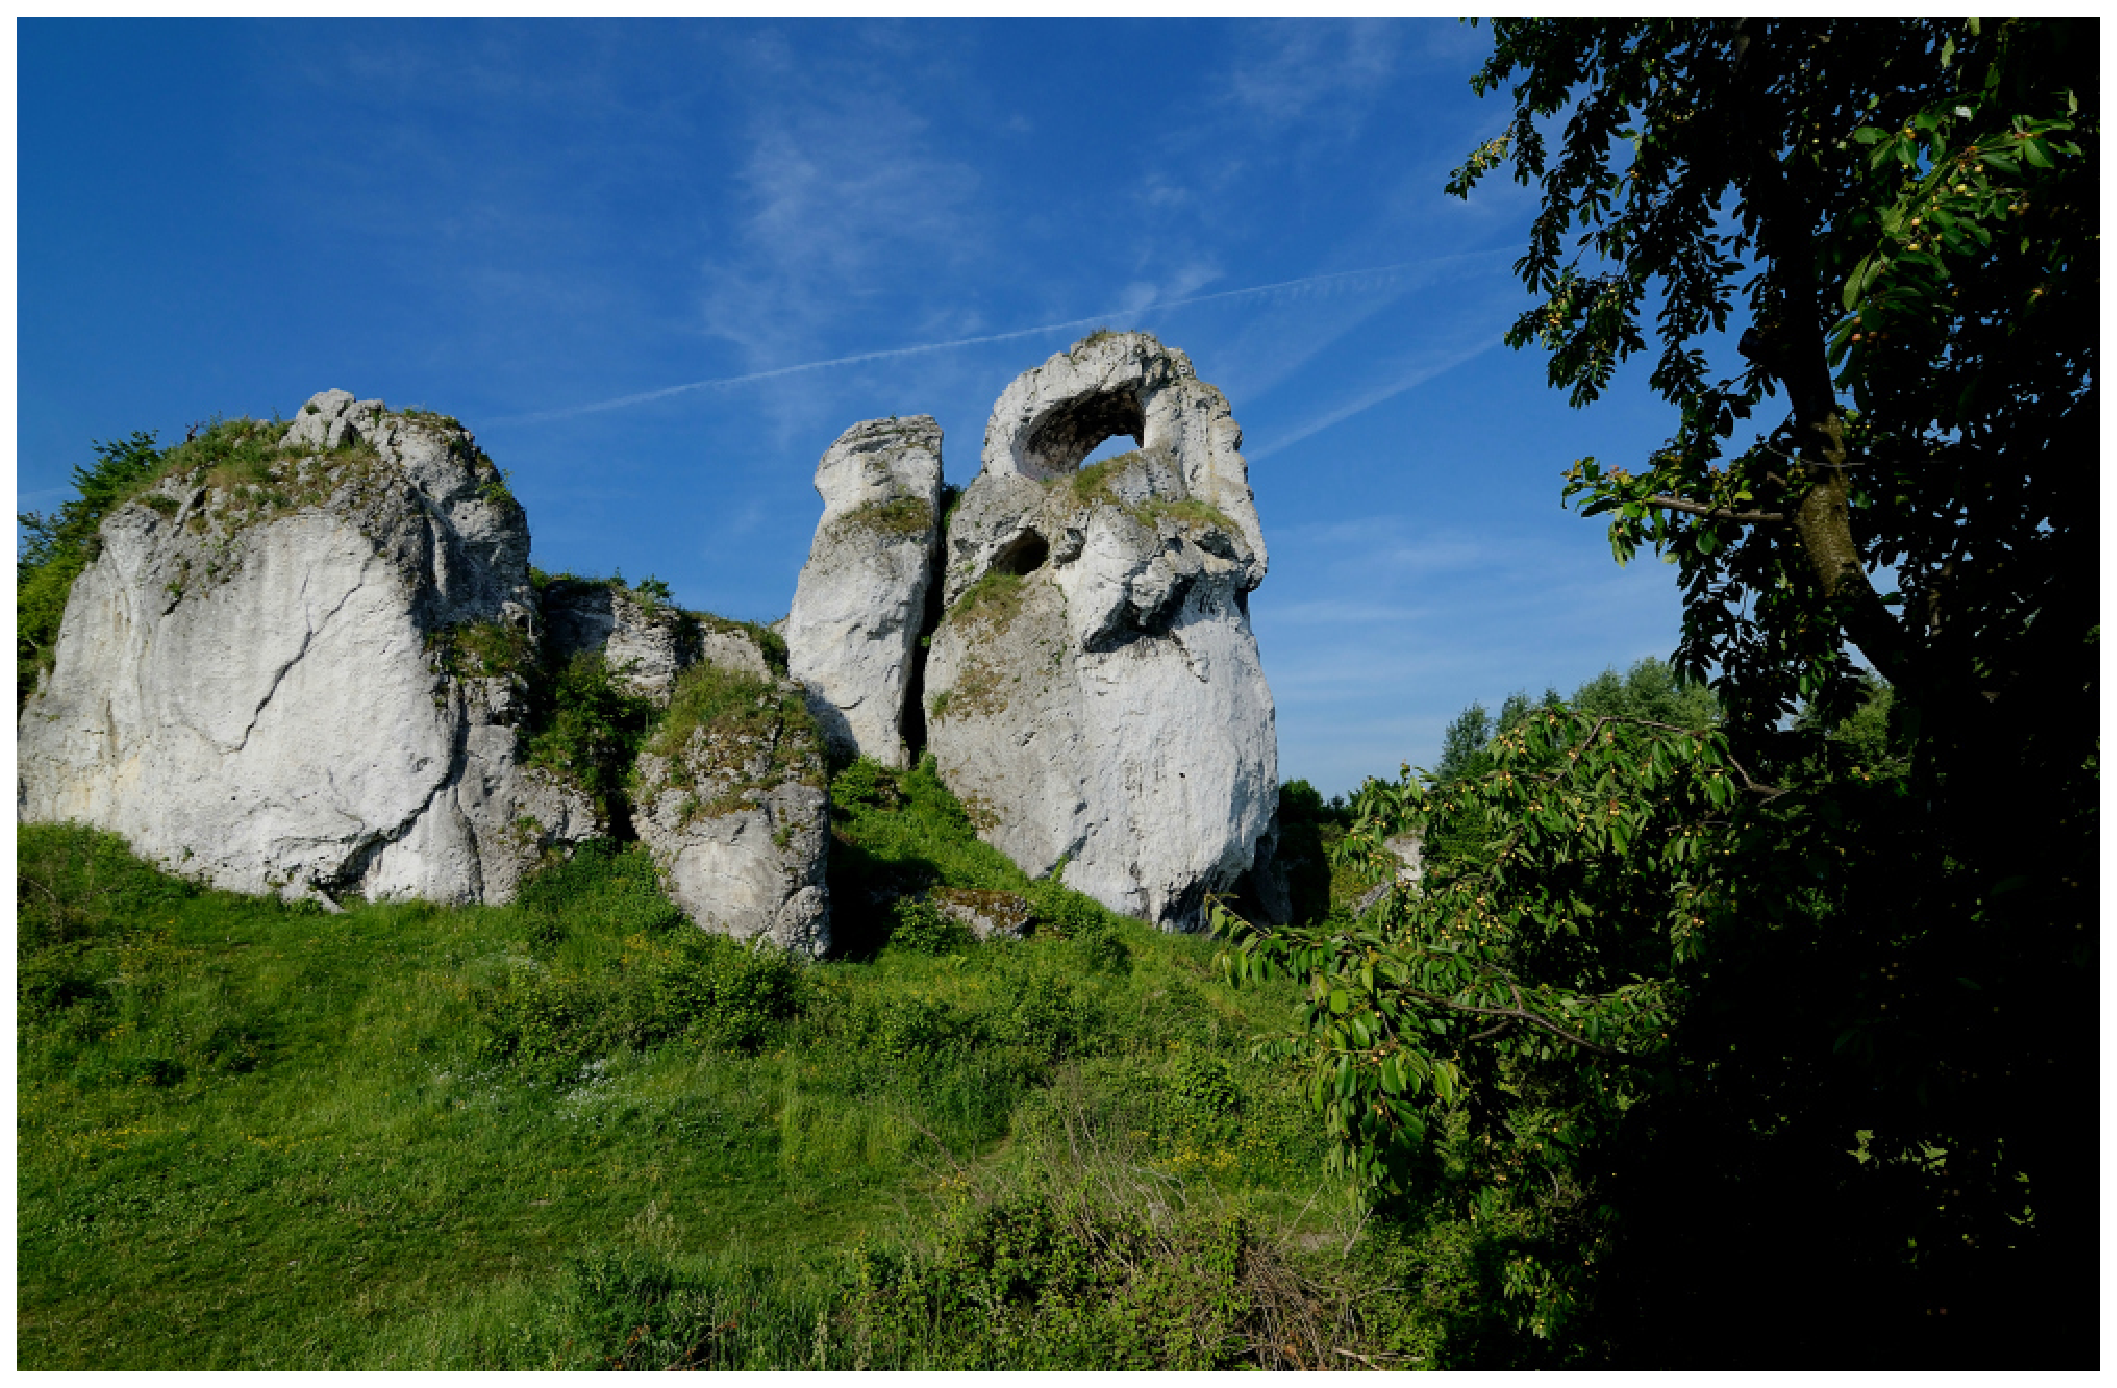
\includegraphics[width=0.9\linewidth]{images/jura-okiennik.eps}
	\end{center}
	\caption{Takie piękne skałki możemy spotkać na Jurze. Główna ściana Okiennika Wielkiego widziana od wschodu (fot. Paweł Wrona)\cite{jura-okiennik}.}
	\label{}
\end{figure}

Jako, że jestem zupełnym amatorem jeśli chodzi o wspinaczkę skałkową, poniżej postaram się przedstawić dwa przykładowe rejony Jury odpowiednie do rozpoczęcia przygody ze wspinaniem \cite{jura-okiennik}. 

\subsubsection{Rzędkowice}
Rzekomo wielu wspinaczu tutaj zaczyna swoją przygodę z Jurą. Jednym z powodów, może być fakt, że początkujący wspinacz znajdzie tutaj ponad 200 linii o wycenie do VI+ włącznie \cite{jura-rzedkowice}. Zdaniem Pawła Wrony z 8academy na początek wspinania w tym rejonie, godnymi uwagi może być skała \textit{Zegarowa} (rysunek \ref{zegarowa}) wraz z trasami \textit{Połupany filarek III} czy \textit{Ostatnią IV+} \cite{jura-rzedkowice}.

\begin{figure}[!htbp]
	\begin{center}
		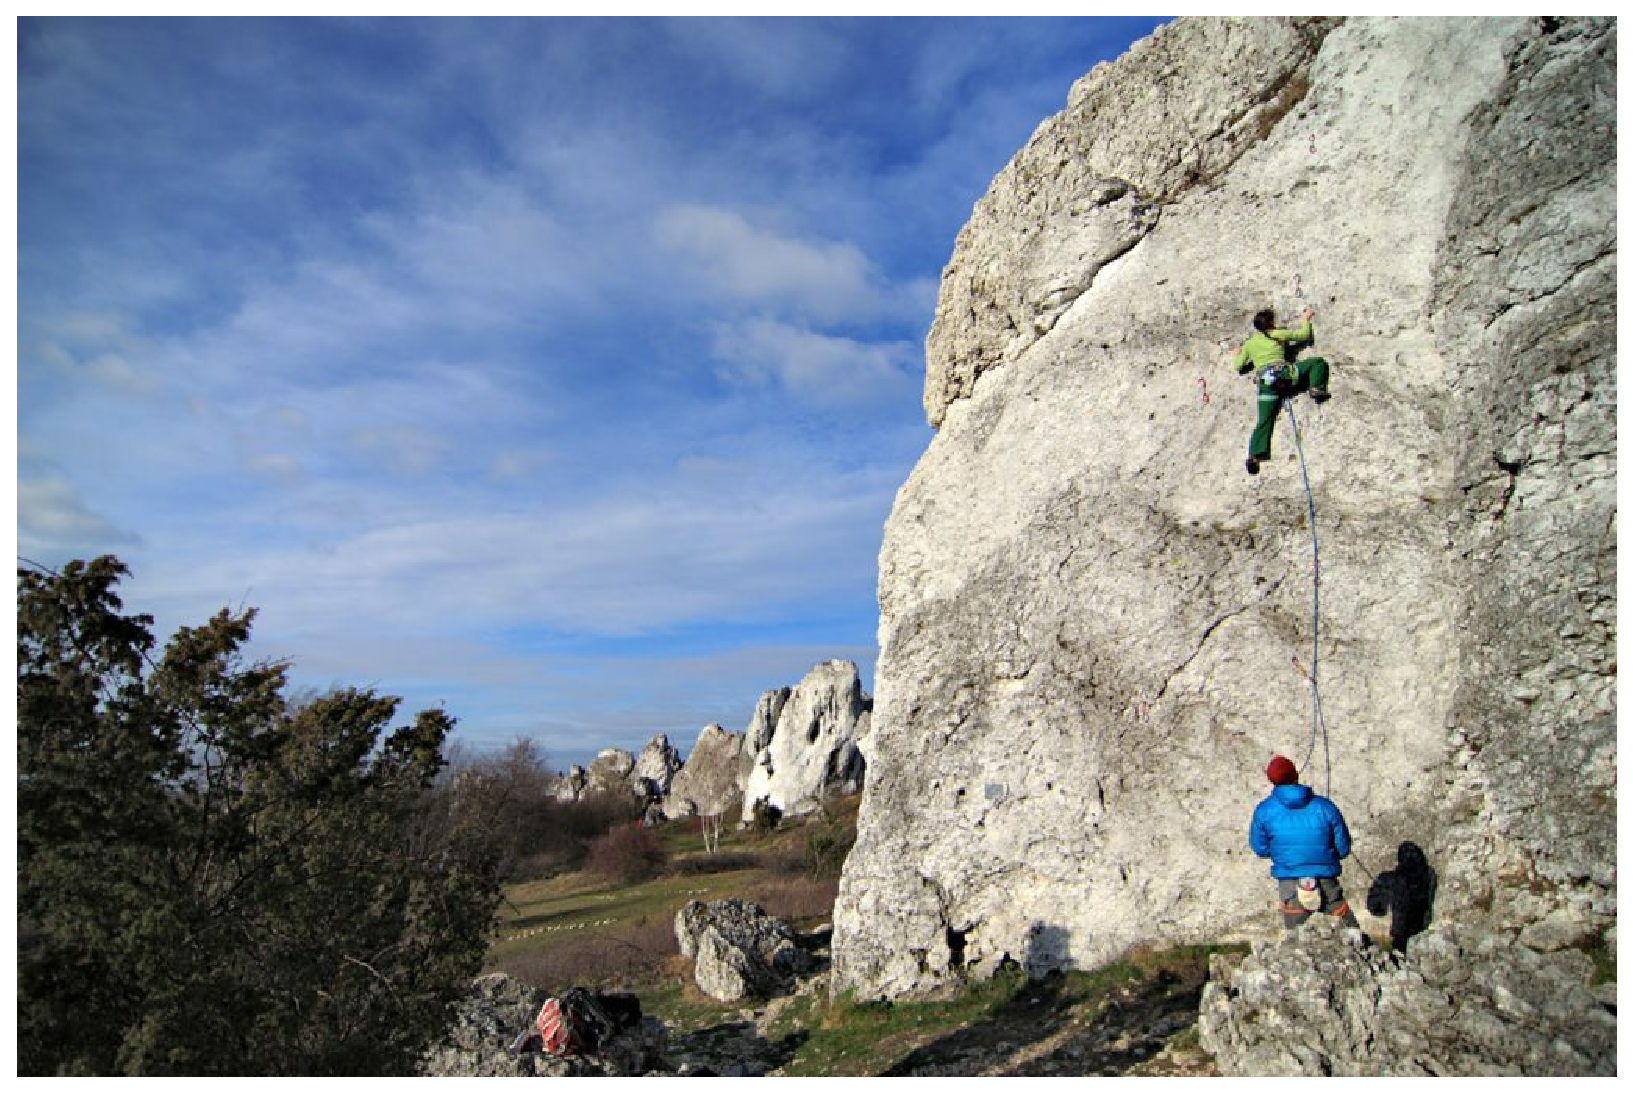
\includegraphics[width=0.9\linewidth]{images/jura-zegarowa.eps}
	\end{center}
	\caption{Wspinanie na Zegarowej, Rzędkowice (fot. Paweł Wrona)\cite{jura-rzedkowice}.}
	\label{zegarowa}
\end{figure}

\subsubsection{Góra Zborów}
Rezerwat Góra Zborów znajduje się w pobliżu miejscowości Podlesice. Znajdziemy tutaj wytyczonych ponad 100 tras wycenionych poniżej VI+ włącznie \cite{topo-gora-zborow}. Początkujący będą mieli zatem z czego wybierać. Ponownie posiłkując się opinią Pawła Wrony, warto na początek rozważyć skałę \textit{Gąsieckiego} z trasami \textit{Dziurki całkiem prawe IV}, \textit{Mały Wachowicz V+} lub \textit{Dziurki VI}. Jeśli chcielibyśmy spróbować czegoś trudniejszego, możemy powspinać się na skale \textit{Młynarz}, gdzie zostały poprowadzone m.in. trasy \textit{Lewy Młynarz VI+} i \textit{Prawy Młynarz VI} \cite{jura-gora-zborow}.

\begin{figure}[!htbp]
	\begin{center}
		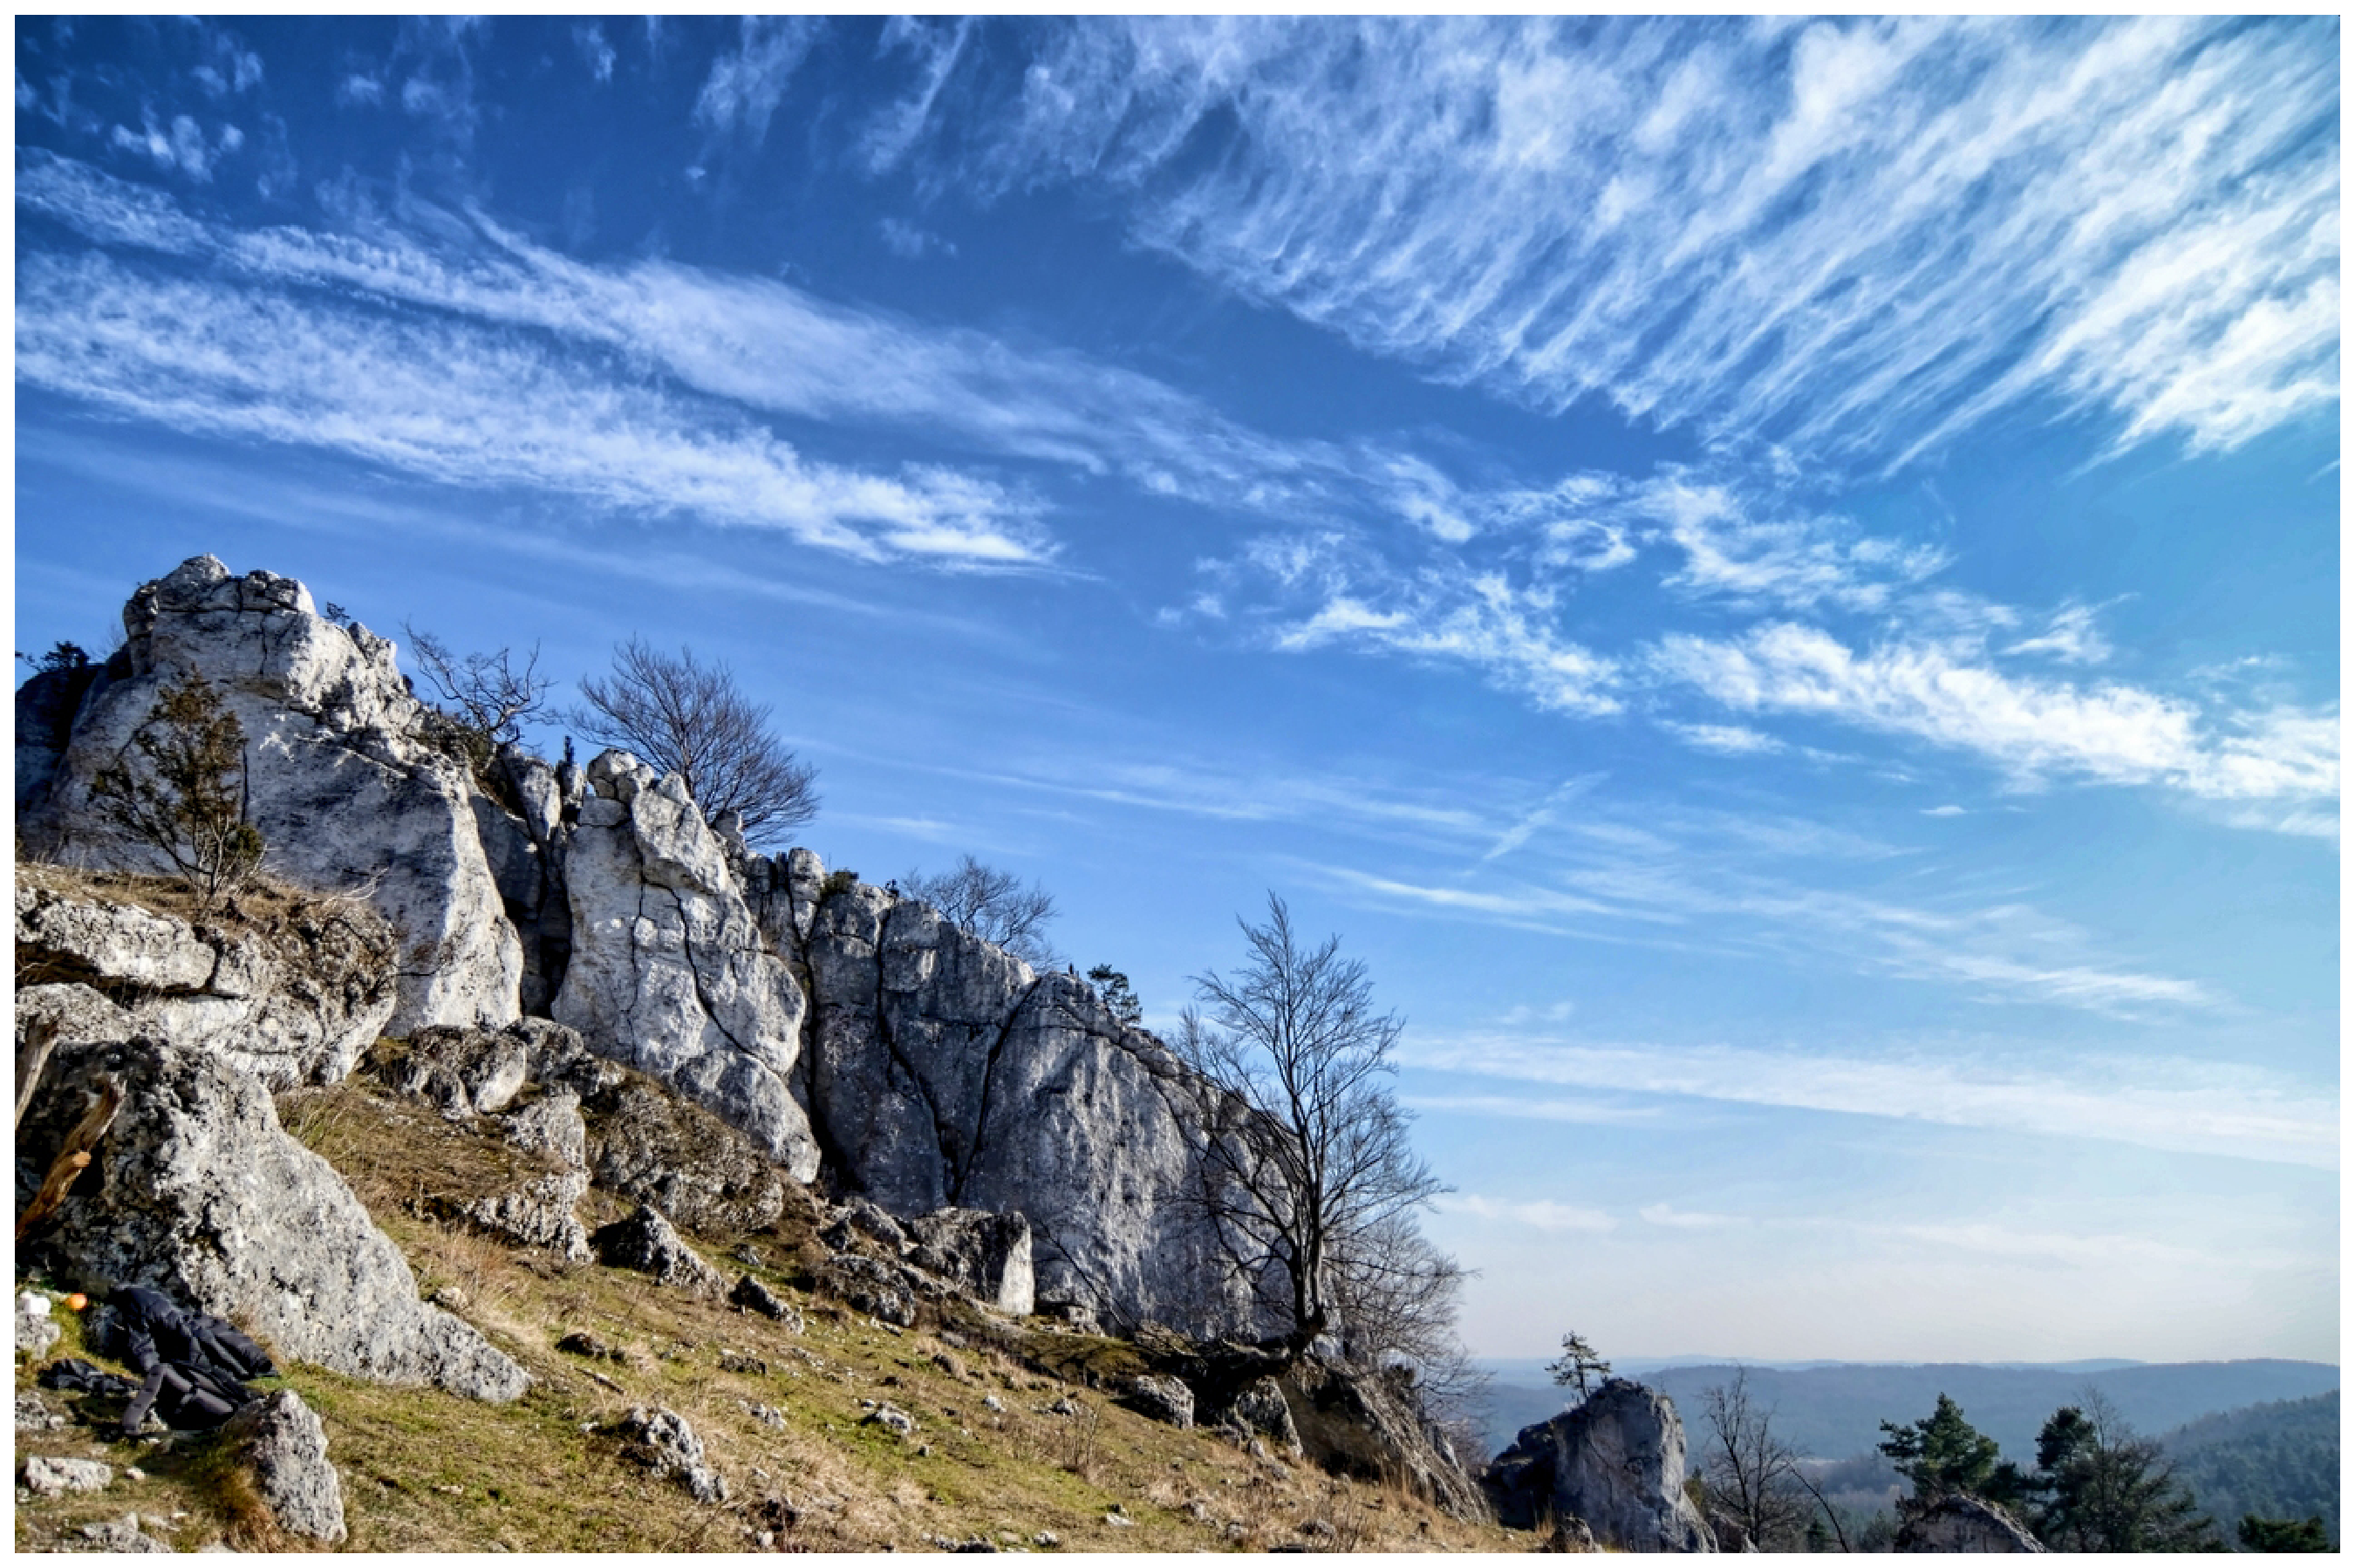
\includegraphics[width=0.9\linewidth]{images/jura-gora-zborow.eps}
	\end{center}
	\caption{Długa grań z widoczną po lewej ścianą \textit{Dziurek} (fot. Paweł Wrona)\cite{jura-gora-zborow}.}
	\label{zborow}
\end{figure}

\begin{figure}[!htbp]
	\begin{center}
		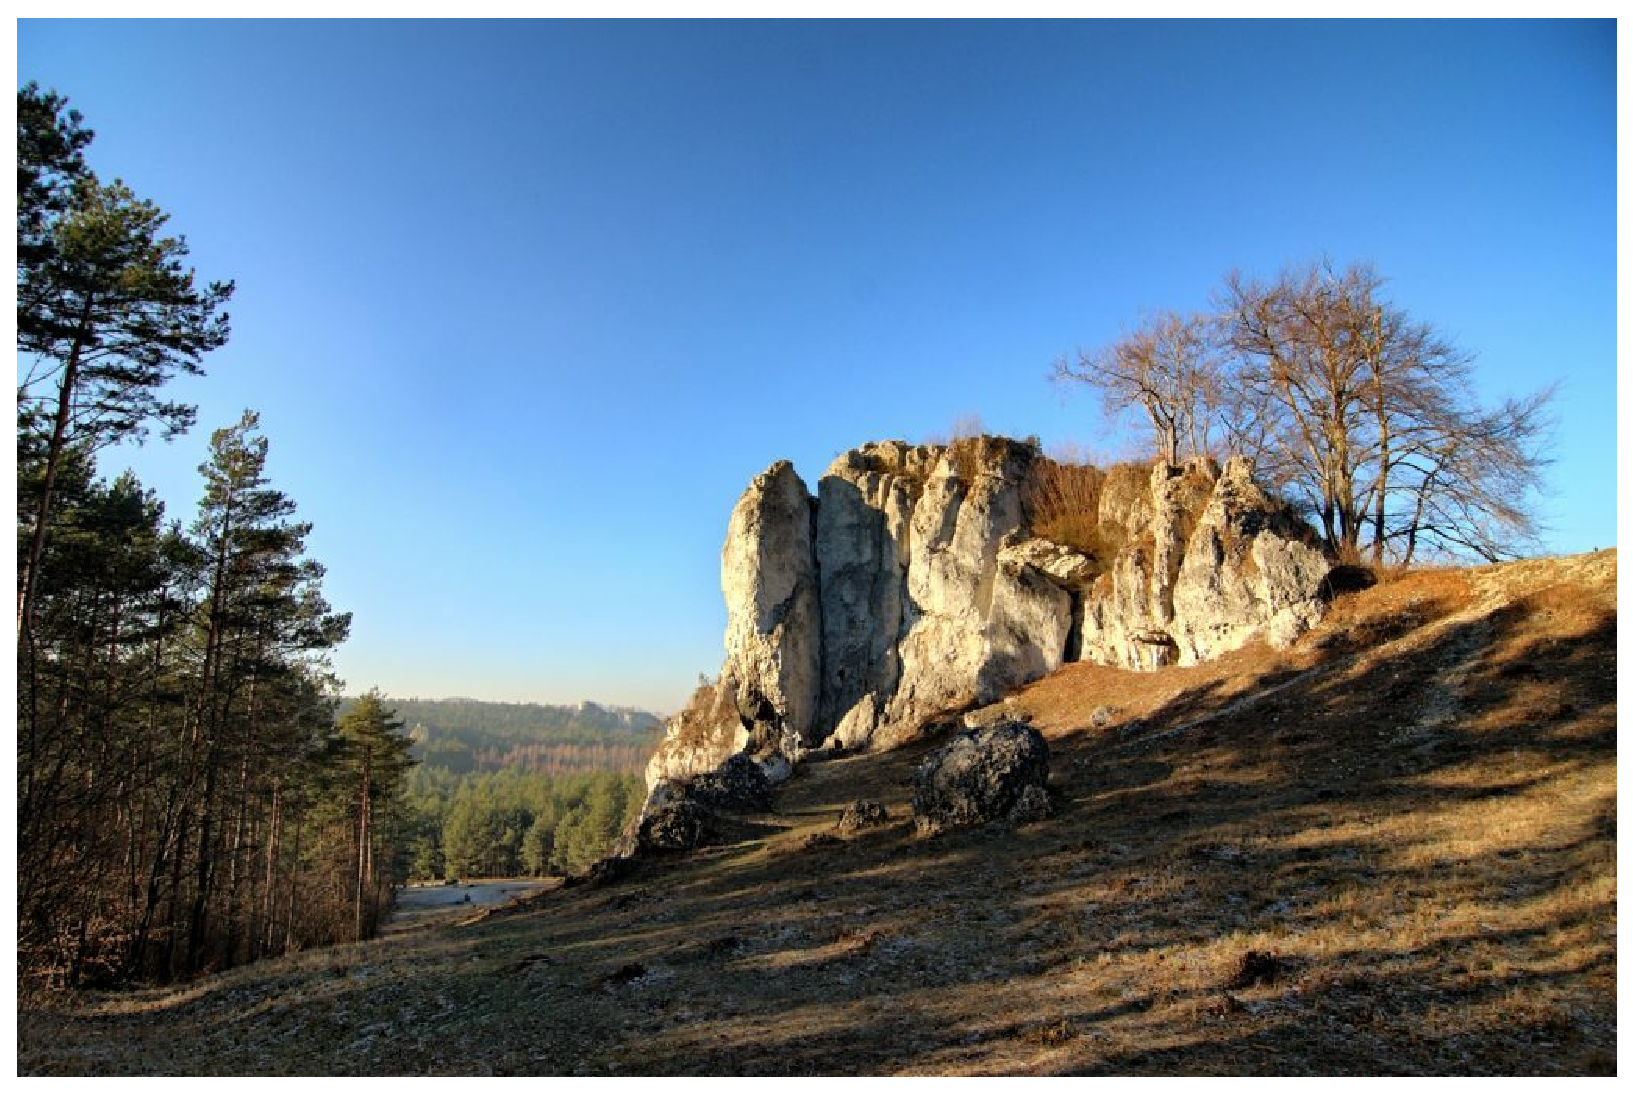
\includegraphics[width=0.9\linewidth]{images/jura-gora-zborow-2.eps}
	\end{center}
	\caption{Okolice Kruka, Góra Zborów (fot. Paweł Wrona)\cite{jura-gora-zborow}.}
	\label{}
\end{figure}

\subsection{Sokoliki}

\subsection{Góry Stołowe}

\pagebreak
\nocite{*}
\addcontentsline{toc}{section}{Bibliografia}
\printbibliography

\end{document}
